\documentclass[../../../include/open-logic-section]{subfiles}

\begin{document}

\olfileid[id]{sth}{ordinals}{idea}
\olsection{Gagasan Umum tentang Ordinal}

Perhatikan bilangan asli dalam urutan lazimnya:
\begin{center}
	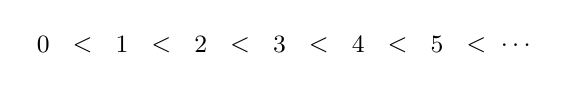
\begin{tikzpicture}
	\foreach \x/\xtext in {0, 1, 2, 3, 4, 5}
	{
		\node (\x a) at (\x, 1) {\small{$\x$}};
		\node (\x a) at (\x.5, 1) {\small{$<$}};
	}
	\node (ldots) at (6, 1) {\small{$\ldots$}};
	\end{tikzpicture}
\end{center}
Dalam istilah teknis, kita menyebutnya barisan-$\omega$. Urutan umum ini
memang tercermin dalam konstruksi awal kita atas tahap-tahap hierarki
himpunan. Namun, sekarang andaikan kita memindahkan~$0$ ke akhir barisan ini,
sehingga bilangan itu berada sesudah semua bilangan lain:
\begin{center}
	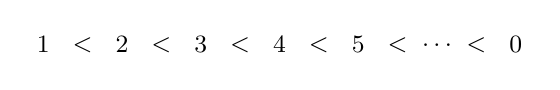
\begin{tikzpicture}
	\foreach \x/\xtext in {1, 2, 3, 4, 5}
	{
		\node (\x a) at (\x, 1) {\small{$\x$}};
		\node (\x a) at (\x.5, 1) {\small{$<$}};
	}
	\node (ldots) at (6, 1) {\small{$\ldots$}};
	\node (bea) at (6.5, 1) {\small{$<$}};
	\node (noa) at (7, 1) {\small{$0$}};
	\end{tikzpicture}
\end{center}
Di sini kita mempunyai entitas-entitas yang sama, tetapi ditata dengan cara
yang secara mendasar berbeda: urutan pertama kita tidak mempunyai anggota
terakhir, sedangkan urutan baru kita mempunyainya. Urutan baru ini terdiri
atas suatu barisan-$\omega$ entitas ($1,2,3,4,5,\ldots$), diikuti satu entitas
lagi. Jadi, urutan ini merupakan barisan-$\omega+1$.

Kita dapat menghasilkan lebih banyak lagi jenis urutan hanya dengan
menggunakan entitas-entitas tersebut. Sebagai contoh, perhatikan semua
bilangan genap (dalam urutan alaminya), diikuti semua bilangan ganjil (dalam
urutan alaminya):
\begin{center}
	\begin{tikzpicture}
	\node(a1) at (1,1) {\small{$0$}};
	\node(a2) at (1.5,1) {\small{$<$}};
	\node(a3) at (2,1) {\small{$2$}};
	\node(a4) at (2.5,1) {\small{$<$}};
	\node(a5) at (3,1) {\small{$4$}};
	\node(a6) at (3.5,1) {\small{$<$}};
	\node(dots) at (4,1) {\small{$\ldots$}};
	\node(aaoe) at (4.5,1) {\small{$<$}};
	\node(b1) at (5,1) {\small{$1$}};
	\node(b2) at (5.5,1) {\small{$<$}};
	\node(b3) at (6,1) {\small{$3$}};
	\node(b4) at (6.5,1) {\small{$<$}};
	\node(b5) at (7,1) {\small{$\ldots$}};
	\end{tikzpicture}
\end{center}
Ini adalah suatu barisan-$\omega$ yang diikuti barisan-$\omega$ lain, yakni
barisan-$\omega+\omega$.

Kita dapat terus melanjutkannya. Namun, yang kita inginkan ialah cara umum
untuk memahami pembicaraan mengenai \emph{urutan} semacam ini.

\end{document}
